
\documentclass[]{spie}  %>>> use for US letter paper
%%\documentclass[a4paper]{spie}  %>>> use this instead for A4 paper
%%\documentclass[nocompress]{spie}  %>>> to avoid compression of citations
%% \addtolength{\voffset}{9mm}   %>>> moves text field down
%% \renewcommand{\baselinestretch}{1.65}   %>>> 1.65 for double spacing, 1.25 for 1.5 spacing 
%  The following command loads a graphics package to include images 
%  in the document. It may be necessary to specify a DVI driver option,
%  e.g., [dvips], but that may be inappropriate for some LaTeX 
%  installations. 
\usepackage[]{graphicx}
\usepackage{float}
\usepackage{subcaption}
\usepackage{amsmath}
\usepackage{enumitem}
\usepackage{multicol}
\usepackage{cleveref}
\usepackage{hyperref}
\usepackage{wrapfig}


\graphicspath{{./images/}}

\title{Federating Heterogeneous Datasets to Enhance Data Sharing and Experiment Reproducibility} 

\author{Juan C. Prieto.\supit{a}, Beatriz Paniagua.\supit{a}, Marilia S. Yatabe.\supit{b}, Antonio C.O Ruellas.\supit{b}, 
Liana Fattori.\supit{b}, Luciana Muniz.\supit{b}, Martin Styner.\supit{a}, and Lucia Cevidanes.\supit{c}
\skiplinehalf
\supit{a}NIRAL, UNC, Chapel Hill, North Carolina, United States; 
\supit{b}DCBIA, UMICH, Ann Arbor, Michigan, United States;
}

%>>>> Further information about the authors, other than their 
%  institution and addresses, should be included as a footnote, 
%  which is facilitated by the \authorinfo{} command.

\authorinfo{Further author information: (Send correspondence to J.C.P)\\J.C.P.: E-mail: jprieto@med.unc.edu}
%%>>>> when using amstex, you need to use @@ instead of @
 

%%%%%%%%%%%%%%%%%%%%%%%%%%%%%%%%%%%%%%%%%%%%%%%%%%%%%%%%%%%%% 
%>>>> uncomment following for page numbers
% \pagestyle{plain}    
%>>>> uncomment following to start page numbering at 301 
%\setcounter{page}{301} 
 
  \begin{document} 
  \maketitle 

%%%%%%%%%%%%%%%%%%%%%%%%%%%%%%%%%%%%%%%%%%%%%%%%%%%%%%%%%%%%% 
\begin{abstract}

Recent studies have demonstrated the difficulties to replicate scientific findings and/or experiments published in past\cite{open2015estimating}. 
The effects seen in the replicated experiments were smaller than previously reported. Some of the explanations 
for these findings include the complexity of the experimental design and the pressure on researches to report positive findings. 
The International Committee of Medical Journal Editors (ICMJE) suggests that every study considered for publication must 
submit a plan to share the de-identified patient data no later than 6 months after publication. 
There is a growing demand to enhance the management of clinical data, facilitate data sharing across institutions and also to keep track 
of the data from previous experiments. The ultimate goal is to assure the reproducibility of experiments in the future.
This paper describes Shiny-tooth, a web based application created to improve clinical data acquisition during the clinical trial; 
data federation of such data as well as morphological data derived from medical images; 
Currently, this application is being used to store clinical data from an osteoarthritis (OA) study. 
This work is submitted to the SPIE Biomedical Applications in Molecular, Structural, and Functional Imaging conference.

\end{abstract}

%>>>> Include a list of keywords after the abstract 

\keywords{Data federation, reproducibility, clinical data, sharing, de-identified, web visualization}

%%%%%%%%%%%%%%%%%%%%%%%%%%%%%%%%%%%%%%%%%%%%%%%%%%%%%%%%%%%%%
\section{INTRODUCTION}
\label{sec:intro}

The primary motivation of this work is to improve the state of clinical research data organization in order to facilitate data sharing across institutions and collaborators and ultimately to facilitate the reproducibility of clinical trials.
A number of issues have been identified when working and managing clinical data recorded during clinical trials funded by the National Institute of Health 
(NIH) or private institutions. Frequently, clinical data is recorded and stored in spreadsheets by the clinicians. Very often, before the data analysis begins, 
a significant amount of time is needed to parse, format and detect outliers in the data in order to produce a dataset suited for analysis.

After the analysis is completed and the results have been published, in the majority of cases, 
the clinical data is not public and/or shared beyond the data holder and collaborators. 
This situation has drawn the attention of the scientific community due to the fact that many scientific findings cannot be easily replicated by other groups. 

As time progresses, the reproducibility of a study decreases for a number of reasons: losing track of the location of the data, the scientist is mutated to another institution and/or the the data needs to be reprocessed. As shown by The Open Science Foundation, in an effort to replicate 100 experiments reported in psychological science during 2008\cite{open2015estimating}, about one-third to one-half of the original findings were also observed in the replication studies. 
Similar patterns can be observed in other areas such as cancer research and engineering. 
After the experiments were replicated, the effects seen were smaller than previously reported. 
Some of the explanations for these findings include the complexity of the experimental design and the pressure on researches to report positive findings. 

Recent guidelines proposed by The International Committee of Medical Journal Editors (ICMJE) suggests that a study considered for publication should 
contain a plan to share the de-identified patient data (IPD) and also supplementary material no later than 6 months 
after publication\cite{doi:10.1001/jama.2015.18164}. The main goal is to improve the transparency and robustness of the publications. 

Today, there is a growing demand to enhance the Clinical Data Management (CDM) \cite{krishnankutty_data_2012} in the scientific community. 
CDM describes the processes to maintain high-quality and reliable data from clinical trials.  
Some of the procedures in CDM include data annotation, database design, data validation etc. 
Recent advancements in web technologies could provide the necessary means to generate publicly available tools and/or services to 
facilitate data sharing across institutions, keep track of data from previous experiments and more importantly to 
assure the reproducibility of experiments in the future.

This paper describes Shiny-tooth, a web based application created to facilitate data 
acquisition during the clinical trial; 
data federation of such data as well as morphological data derived from medical images; 
interactive visualization of the clinical and morphological data; and task submission 
to remote computing grids using the data stored in the system.

For data storage, we use couchdb, a NoSQL database that uses Javascript Object Notation 
(JSON) format to store documents 
and offers a document-based query and indexing mechanism
Additionally, couchdb allows attaching binary data to the documents, i.e., medical images, tessellations, etc.; it is implemented following Representational State Transfer (REST) architecture to insert, modify, retrieve and delete records; 
and offers a synchronization feature between two couchdb instances.
Additional frameworks have been used to develop the application, the following section describes 
the application's architecture. 

Currently, this application is being used to store clinical data from an osteoarthritis (OA) study. OA is the most prevalent arthritis worldwide, is associated with significant pain and disability and affects 13.9\% of adults at any given time. OA is very complex and the pathogenesis of TMJ OA remains unclear to this day. OA affects the temporomandibular joint (TMJ), among other joints. TMJ OA represents 42.6\% of the diagnosed disorders of the TMJ, and results in \$4 billion annual health care costs in the US\cite{Cevidanes2010110}\cite{Paniagua2011345}. 
In the future we expect to create repositories to study rare diseases such as OA and facilitate anonymized data sharing
across institutions.

\section{METHODS} 
\label{sec:METHODS}

Shiny-tooth is focused on the re-usability of components and creating a robust and scalable application. 

The back-end of the application is built using Node.js\footnote{\url{https://nodejs.org}},
Hapi.js\footnote{\url{http://hapijs.com/}}, Couchdb\footnote{\url{http://couchdb.apache.org}} and 
user authentication is done with Json Web Tokens (JWT)\footnote{\url{https://jwt.io}}. 

The front-end of the application is build using Angular.js\footnote{\url{https://angularjs.org}}, 
Data Driven Documents (D3.js)\footnote{\url{https://d3js.org/}} and 
Three.js\footnote{\url{https://threejs.org/}} for 3D visualization. 

Additionally, a plug-in for 3DSlicer\footnote{\url{https://www.slicer.org}} 
is implemented to commit and retrieve data directly 
from the system. 

The following sections gives additional detail about the tools used to build this system. 

\subsection{Back-end framework}

Node is a Javascript engine that facilitates building 
scalable network applications. 
Using Hapi as the server framework, we are able to build 
services and focus on writing reusable application logic instead 
of pure infrastructure. 
Hapi is fully REST and orchestrates communication between all components in the system.
The tool used for storage is Couchdb, a NoSQL type database, i.e., 
it does not store data and relationships in tables. Instead, 
each database is a collection of independent JSON documents. JSON is a flexible format 
and facilitates encoding data without enforcing a predefined rigid structure. 

For our application, storing data in such format presents an advantage
as we don't know beforehand the structure of incoming data. 
Once the data is stored in the system, the relationships between documents are discovered using 
the map reduce algorithm and generating views indexing the data in the system. 

User authentication is handled with JWT. A plug-in 
is developed allowing storage and retrieval of user information, as well 
as JWT encryption exchanged with the user upon login. 

Finally, clusterpost\footnote{\url{https://www.npmjs.com/package/clusterpost-provider}} is
integrated in the system. This plug-in allows 
submitting tasks to remote computing grids using the data stored in the system.

\subsection{Front-end framework}

The front end of the application is based on Angular.js, this framework facilitates the development of reusable HTML components.
The clinical data visualization is done using D3.js and 3D visualization of morphological data is accomplished with Threejs.
The application is hosted using Amazon web services or the Elastic Computing Cloud (EC2). Shiny-tooth has been applied to store clinical OA data. 

\subsection{3D Slicer plug-in}

3D Slicer is an open source software for 3D image processing and visualization. 
It is known as the "Swiss knife" for medical images as it provides 
several tools to manipulate them.
Furthermore, it allows software developers to contribute plug-ins and 
Slicer users to install them via an extension manager. 

We have developed a Slicer extension
that enables clinicians to download and upload 
data directly to shiny-tooth server. Additionally, 
we have implemented the interface to use clusterpost and 
submit high intensive computational tasks to remote computing grids. 

\section{MATERIALS}

The current study consists of 218 TMJ joints, (153 TMJ OA, 65 Controls) obtained from CBCT 
images. 

Label maps of the TMJs were generated and point distribution models (PDM) with 1002 correspondent 
points were constructed using SPHARM-PDM\cite{Styner2006}. 

Previously acquired clinical and biological data 
is added to the repository. 
Incoming data is being recorded directly in the system via study specific questionnaires.

\section{RESULTS} 

Figure \ref{fig:serverArchitectureOut} shows the architecture of the application and 
the plug-ins deployed in the system.

\begin{figure}
	\centering 
	\includegraphics[width=14cm]{serverArchitectureOut.eps}
	\caption[Server architecture]{Server architecture based on plugins for a distributed application. 
	The framework allows easy integration of a variety of plug-ins. The authentication system is based on JSON Web Tokens. 
	The clusterpost plug-in allows submitting heavy computational tasks to remote computing grids.}
	\label{fig:serverArchitectureOut}
\end{figure} 

Figure \ref{fig:gnerateClinicalData} shows the procedure to create data for the current clinical study. 
\ref{fig:gnerateClinicalData}.a shows a collection of Biological Markers. A Collection in this system is defined as a group of clinical data. Nevertheless, 
each JSON document is indexed separately and may be retrieved using the document's content. A collection may be utilized to facilitate the retrieval of meaningful datasets in a study. \ref{fig:gnerateClinicalData}.b shows an extract from a form used to acquire patient information. 
\ref{fig:gnerateClinicalData}.c displays the clinical data in a table format. Another feature of the system is the possibility to import previously acquired data in spreadsheets. However, the content of the spreadsheet must be converted to a comma separated value (CSV) format with the first row being the table header. The header or column names will be used to index the data in the future. If the data is imported from a spreadsheet, it is necessary to specify the column that contains the anonymization id. This id will be used to index the JSON document and perform joints between clinical and morphological data.

\begin{figure}
	\centering 
	\begin{subfigure}{0.3\textwidth}
		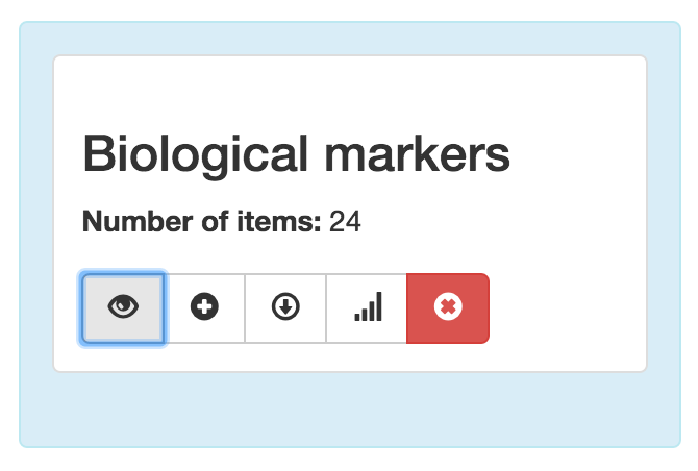
\includegraphics[width=5.5cm]{CreateCollectionsOut.eps}
		\caption{}
    	\label{fig:CreateCollections}
	\end{subfigure}
	\begin{subfigure}{0.3\textwidth}
		\includegraphics[width=3cm]{inputFormStructuredDataOut.eps}
		\caption{}
    	\label{fig:inputFormStructuredData}
	\end{subfigure}
	\begin{subfigure}{0.3\textwidth}
		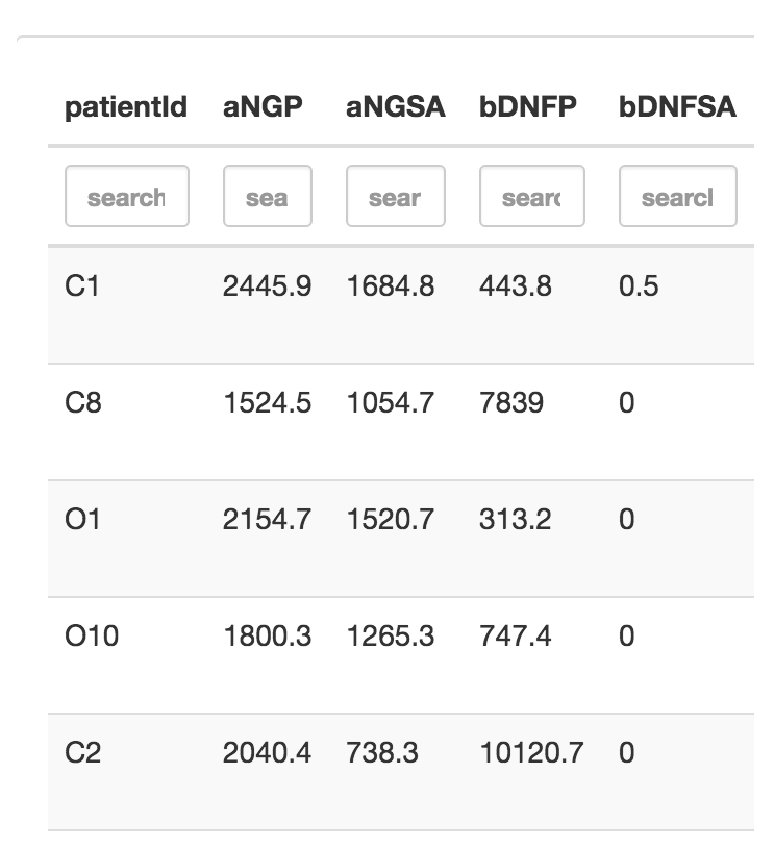
\includegraphics[width=3cm]{ImportDataFromSpreadSheetsOut.eps}
		\caption{}
    	\label{fig:ImportDataFromSpreadSheets}
	\end{subfigure}
	\caption[Import and generate clinical data]{a) Create a group or collection for clinical data. b) Forms or questionnaire. c) clinical data visualization.}
	\label{fig:gnerateClinicalData}
\end{figure} 

Figure \ref{fig:queryAndSelect}.a shows a view where the user can select different clinical variables, in this case, the variables correspond to genetic data
acquired for this study. Figure \ref{fig:queryAndSelect}.b shows patient selection. Figure \ref{fig:queryAndSelect}.c shows a plot using the selected 
variables in the clinical data and patient section. 

\subsection{3DSlicer plug-in}

We have developed a plug-in to facilitate interaction with the system 
directly from one of the most popular software for medical image processing and three-dimensional visualization. 
3DSlicer is used by many research groups worldwide, is open-source, and provides a wide range 
of processing tools to physicians, researchers, and the general public. 



This extension contains multiple panels that allow the user to manage data from a CouchDB database stored on a server. It has been developed to work with this website, so the user will need to have an account on this website. The data currently stored on this website is for a pilot study which needs to federate biological, morphological and clinical data. At the end of the development of the website, this should be available for other projects. For more information about the website status, contact .
The data displayed in this extension dynamically reacts with user local folders and online database. The user should login with the same credentials than on the server entered as input.

\begin{figure}
	\centering 
	\begin{subfigure}{0.3\textwidth}
    	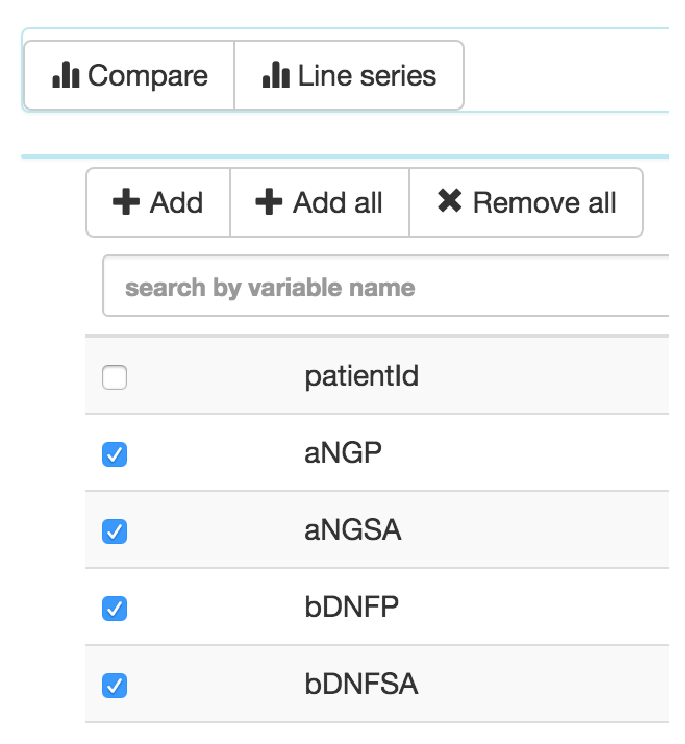
\includegraphics[width=\textwidth]{QueryAndFilterImportedDataOut.eps}
    	\caption{Query and filter data}
    	\label{fig:QueryAndFilterImportedData}
	\end{subfigure}
	\begin{subfigure}{0.3\textwidth}
    	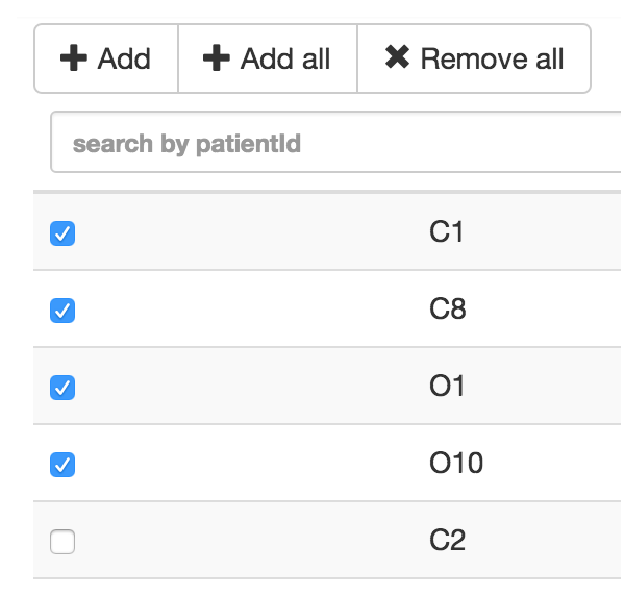
\includegraphics[width=\textwidth]{SelectPatientsOut.eps}
    	\caption{Select control patients}
    	\label{fig:SelectPatients}
	\end{subfigure}
	\begin{subfigure}{0.3\textwidth}
    	\includegraphics[width=\textwidth]{PlotOfControlPatientsForSomeProteinsOut.eps}
    	\caption{Plot proteins for patients}
    	\label{fig:PlotOfControlPatientsForSomeProteins}
	\end{subfigure}
	\caption[Import and generate clinical data]{a) Query and select clinical data. b) Query and select patients. c) Plot the selected data}
	\label{fig:queryAndSelect}
\end{figure}

The plot produced in figure \ref{fig:queryAndSelect}.c is an interactive plot where the user can select a line and/or the legend on top 
in order to retrieve morphological data from the database. Figure \ref{fig:3DVisualizationOfCondyle} shows a drop down menu that is populated 
with the patient's data and the visualization of the structure in the interactive 3D viewer.

\begin{figure}
	\centering 
	\includegraphics[width=7cm]{3DVisualizationOfCondyleOut.eps}
	\caption[Visualization]{Condyle visualization in 3d}
	\label{fig:3DVisualizationOfCondyle}
\end{figure}

\section{CONCLUSIONS} 

The current state of the application allows gathering clinical data and morphological data in a structured manner. 
The tools and plugins described shown in Figure \ref{fig:serverArchitectureOut} have been 
published%\footnote{\url{https://www.npmjs.com/~juanprietob}} 
and are available for installation with the node package manager (npm). 
The current implementation of shiny-tooth has been deployed in the EC2 container and is available 
here%\footnote{\url{https://ec2-52-42-49-63.us-west-2.compute.amazonaws.com:8180}}. 
The access to the data is restricted and will only be allowed after authorization from the project managers. 

%\acknowledgments

%%%%%%%%%%%%%%%%%%%%%%%%%%%%%%%%%%%%%%%%%%%%%%%%%%%%%%%%%%%%%
%%%%% References %%%%%

\scriptsize
\bibliography{report}   %>>>> bibliography data in report.bib
\bibliographystyle{spiebib}   %>>>> makes bibtex use spiebib.bst

\end{document} 
